\section{Insert-Closest-Verfahren} \label{sec:insert-closest-verfahren}
    % Was ist das Min-Dist-Verfahren
        % Umgekehrtes Prinzip von Insert Furthest
        % Allerdings wird nun die nächste Node an den Graphen angehängt
    % Wie funktioniert das Min-Dist-Verfahren
        % Zuerst wird die Node in den Graphen eingefügt, welche den niedrigsten Index im Node Array hat (also am Anfang steht)
        % Dann nun wird die Node gesucht, welche am Nächsten an der ersten Node ist
        % Dazu wird einfach durch alle Nodes iteriert, die Entfernungen berechnet und dadurch die Node mit der geringsten Entfernung ermittelt
        % Diese wird dann an den Graphen angehängt, das heißt in die erste leere Stelle eingefügt
    \subsection{Funktionsweise}
Aufbauend auf den durch das Insert-First- und Insert-Furthest-Verfahren gewonnen Erkenntnissen ist es mögliche weitere Variationen der Heuristik zu entwickeln und deren Ergebnisse zu betrachten.
Da sowohl in \vref{sec:insert-first-verfahren} als auch in \vref{sec:insert-furthest-verfahren} festgestellt wurde, dass ein Grund für suboptimal erstellte Routen die Reihenfolge der Betrachtung der Knoten ist, wird für das Insert-Closest-Verfahren eine weitere anderes Kriterium für eben diese Reihenfolge festgelegt.
Wie der Name des Verfahrens schon suggeriert, geschieht hier die Auswahl der Knoten wieder nach ihrer Distanz.


Das Insert-Closest-Verfahren bezeichnet im Grundprinzip die Umkehrung des Insert-Furthest-Prinzips. 
Anstatt des am weitesten entfernten Knotens wird hier der dem aktuellen Knoten nächste betrachtet.
\\
Zu Beginn beschreibt sich der Algorithmus identisch zum Insert-Furthest-Verfahren.
Auch hier wird ein neuer Graph mit einem leerem Pfad \lstinline{path} und einer Liste von Knoten $k_1, \dots ,k_n$ der Länge $n$ erzeugt.
Auch hier wird der erste Knoten $k_1$ als erster Knoten des Pfades festgelegt.
Der als nächstes einzufügende Knoten wird wie beim Insert-Furthest-Verfahren durch seine Distanz zum vorherigen bestimmt.
Für das Insert-Closest-Verfahren wird der dem Vorherigen Knoten nächste Knoten, unter der Bedingung, dass dieser nicht bereits Teil des Graph ist, in den Pfad eingefügt.
Um die beste Stelle zum Einfügen des Knotens zu ermitteln wird das gleiche Verfahren wie bei den beiden vorherigen Algorithmen angewandt; die Stelle, die den geringsten Anstieg für die Gesamtdistanz des Pfads wird ausgewählt.
Auch das Vorgehen beim Einfügen orientiert sich hier an den vorherigen Algorithmen.
Der aktuelle Knoten $k_i$ wird nach dem in \vref{alg:merge-node-into-path} dargestelltem Prinzip an dem vorher festgelegten Index $j$ in den Graph eingefügt.
\\
Der beschriebene Algorithmus befindet sich als Pseudocode in etwas ausführlicher Version unter \ac{Alg.} \vref{alg:insert-furthest}.
\begin{algorithm}
    \caption{Insert-Closest-Algorithmus}
    \label{alg:insert-closest}
    \begin{algorithmic}[1]
        \Require Graph $G$, Pfad $P$
        \Require $G = k_1,k_2,\ldots,k_n$, $n > 2$
        \State $p_1 \gets k_1$
        \Comment Setzen des ersten Knoten
        % Find furthest
        \State $i \gets -1$
        \State $d_i \gets -1$

        \For{$a \gets 1$, $a \leq n$, $a \gets a + 1$}
            % Main Loop
            % find Furthest from last
            \State $j_S \gets -1$
            \State $d_S \gets -1$

            \For{$b \gets 2$, $b \leq n$, $b \gets b + 1$}
                \Comment Finde $k_b$ mit der geringsten Distanz zu $p_m$
                \State $d_C \gets \omega$($k_b$, $p_m$)
                \Comment Distanz zwischen $k_b$ und letztem Knoten $p_m$
                \If{$k_b \not \in P$ \textbf{and} ($j_S = -1$ \textbf(or) $d_C > d_S$)}
                    \State $d_S \gets d_C$
                    \State $j_S \gets b$
                \EndIf
            \EndFor

            \State $i_S \gets -1$
            \State $d_S \gets -1$

            \For{$b \gets 2$, $b < n$, $b \gets b + 1$}
                \State $d_C \gets$ \textsc{mergeAt}($P$, $b$, $k_{j_F}$) \textsc{distance}
                \If{$i_S = -1$ \textbf{or} $d_C < d_S$}
                    \State $i_S \gets b$
                    \State $d_S \gets d_C$
                \EndIf
            \EndFor
            \State $P \gets$ \textsc{mergeAt}($P$, $k_{j_S}$, $i_S$)
            \Comment Siehe Alg. \vref{alg:merge-node-into-path}
        \EndFor \\
        \Return new Graph($P$)
    \end{algorithmic}
\end{algorithm}

\subsection{Zeitkomplexität}
Da es sich beim Insert-Closest-Algorithmus im eine Abwandlung des Insert-Furthest handelt, ist die Struktur beider Algorithmen gleich -- nur eine Bedingung ändert sich.
Daher kann auch für diesen Algorithmus eine Zeitkomplexität von 
$$f(n) = O(n^2)$$ 
angenommen werden, womit auch dieser Algorithmus wie Insert-First skaliert.

\subsection{Ergebnis und Schwächen}
Auch die Ergebnisse dieses Algorithmus gestalten sich sehr divers.
Wie bei den beiden anderen Verfahren entstehen hier Graphen, die nahe an die Optimale Route heranreichen oder ihr teilweise auch entsprechen, aber auch solche, die weit von der optimalen Lösung abweichen.
Übergibt man dem Algorithmus beispielsweise die gleichen Knoten wie in Abbildung \vref{fig:insert-first-bad}, einem Szenario, bei dem der Insert-First Algorithmus einen suboptimalen Graph generiert, kommt der Insert-Closest Algorithmus, so wie der Insert-Furthest Algorithmus auch, auf die optimale Route.\\
So wie die anderen Algorithmen stößt aber auch der Insert-Closest Algorithmus bei bestimmten Konstellationen von Knoten an seine Grenzen.

\begin{figure}
    \begin{center}
        \subfloat[$m=4$ \label{subfig:insert-closest-BAD-4}]{
            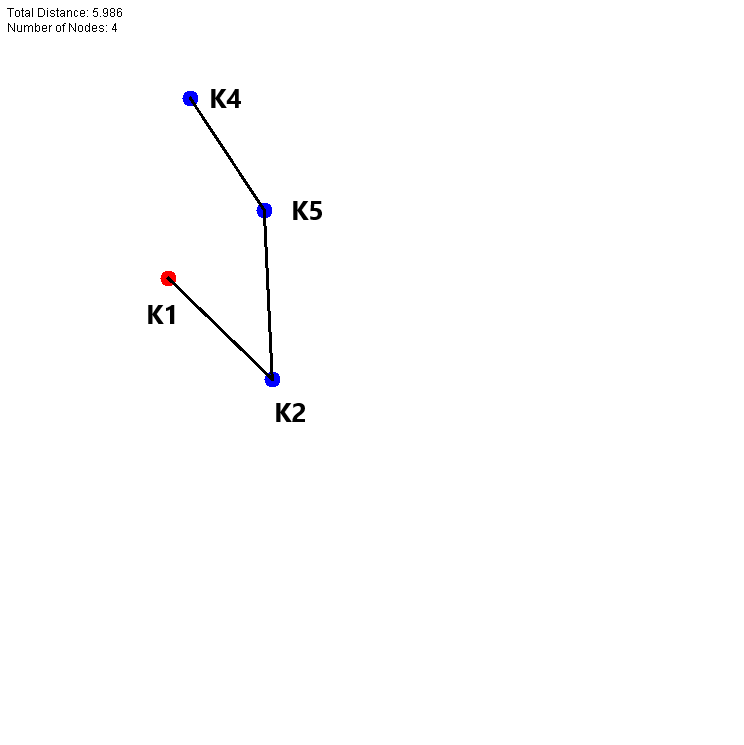
\includegraphics[width=0.35\textwidth]{Bilder/insertClosest/insert_closest_ex_BAD_4.PNG}
        }
        \hfil
        \subfloat[$m=5$ \label{subfig:insert-closest-BAD-5}]{
            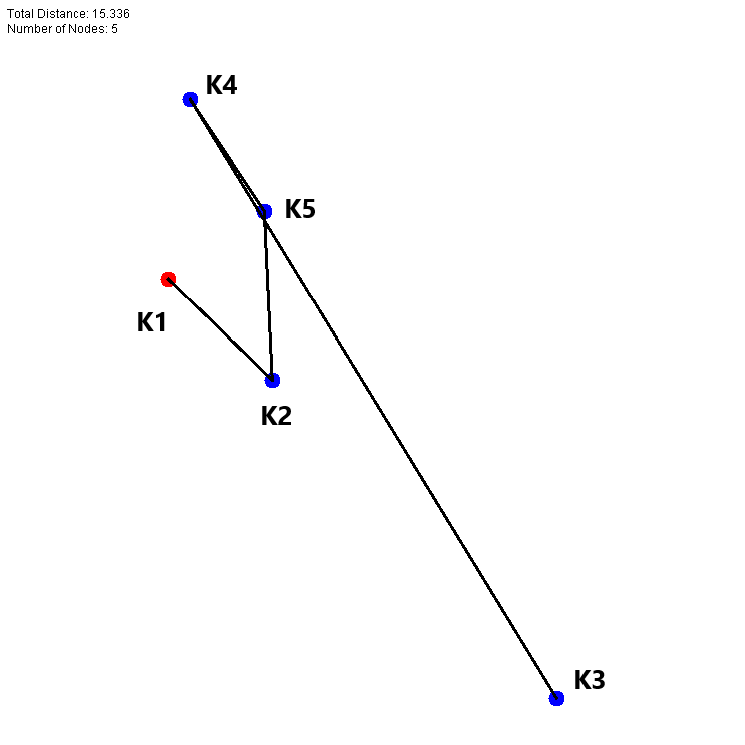
\includegraphics[width=0.35\textwidth]{Bilder/insertClosest/insert_closest_ex_BAD_5.PNG}
        }
        \caption{Der Insert-Closest Algorithmus kommt zu einem schlechten Ergebnis}
        \label{fig:insert-closest-BAD}
    \end{center}
\end{figure}

Wie in Abbildung \vref{fig:insert-closest-BAD} zu sehen ist, plant der Algorithmus einen Pfad, der deutlich erkennbar nicht optimal ist.
Die einzelnen Schritte, die zur Generierung des Graphen führen finden sich im Anhang in der Abbildung \vref{app:fig:insert-closest-BAD-complete}.
Der in \vref{subfig:insert-closest-BAD-5} gezeigt Pfad hat eine Gesamtdistanz von 15,336 \ac{LE}.
Durch das Ändern der Reihenfolge der Knoten zu
% \begin{addmargin}[1em]{2em}
    $$P=k_1, k_4, k_5, k_2, k_3$$ 
% \end{addmargin}
könnte eine Verringerung der Distanz im Vergleich zum vorherigen Resultat um 3,208 \ac{LE}, bzw. 20,918\% erreicht werden.
Auch hier wird der suboptimal geplante Pfad durch die Reihenfolge der Betrachtung der Knoten verursacht.
Im konkreten Beispiel werden die ersten vier Knoten $k_1, k_2, k_4$ und $k_5$ zu einem für sich optimalen Pfad zusammengefügt.
$k_3$ wird aufgrund seiner hohen Distanz zu den übrigen Knoten als letztes in den Pfad eingefügt.
Im gezeigten Beispiel kommt es also genau zu der Umkehrung des Problems, welches beim Insert-Furthest Algorithmus besteht; dort werden Knoten aufgrund ihrer zu niedrigen Distanz teilweise zu spät eingefügt.
Diese Problem hat hier zur Folge, dass $k_3$ als letzter Knoten des Pfads nach dem von ihm am weitesten entfernten Knoten eingefügt wird, was zu einem hohen Zuwachs der Gesamtdistanz führt.